\documentclass[a4paper, 12pt, hidelinks]{article}

\title{Honours Project Dissertation}
\author{Joe Barrett}

\usepackage[natbibapa]{apacite}
\bibliographystyle{apacite}
\usepackage{blindtext}
\usepackage{booktabs}
\usepackage[ddmmyyyy]{datetime}
\usepackage{enumitem}
\usepackage{eurosym}
\usepackage{fancyhdr}
\usepackage{fontspec}
\usepackage[margin=1in]{geometry}
\usepackage[toc,acronym,nonumberlist]{glossaries}
\usepackage{graphicx}
\usepackage{hyperref}
%\usepackage[none]{hyphenat}
\usepackage[nottoc,notlot,notlof]{tocbibind}
\usepackage[table]{xcolor}
\usepackage{url}
\usepackage{verbatim}
\usepackage{pdflscape}
\usepackage{tabularx}
\usepackage{minted}

\setmainfont{Arial}
\pagestyle{fancy}
\renewcommand{\headrulewidth}{0pt}

\lhead{Joe Barrett - 40117680}
\rhead{SOC10101 Honours Project}
\lfoot{}
\cfoot{}
\rfoot{\thepage}

\makeglossary
\loadglsentries{glossary}

\newlist{chapterList}{enumerate}{1}
\setlist[chapterList]{label=\bfseries Chapter \arabic* - }
\newenvironment{where}{\noindent{}where\begin{itemize}[label={}, nosep]}{\end{itemize}}

\begin{document}
	\urlstyle{same}
	\pagenumbering{roman}
	\setcounter{secnumdepth}{4}
	\setcounter{tocdepth}{3}
	\begin{titlepage}
	\begin{center}
		
		\vspace*{3cm}
		{\LARGE Calculation of Mountain Bike Suspension Settings through Image Analysis}
		
		\vspace{3cm}
		{\large Joe Barrett - 40117680}

		\vfill
		Submitted in partial fulfilment of the requirements of Edinburgh Napier University for the Degree of BEng (Hons) Software Engineering
		
		\vspace{1cm}
		School of Computing
		
		\vspace{1cm}
		\today
	\end{center}
\end{titlepage}
	\thispagestyle{empty}
\section*{Authorship Declaration}
I, Joe Barrett, confirm that this dissertation and the work presented in it are my own achievement.
\\\\
Where I have consulted the published work of others is always clearly attributed.
\\\\
Where I have quoted from the work of others, the source is always given. With the exception of such quotations this dissertation is entirely my own work.
\\\\
I have acknowledged all main sources of help.
\\\\
If my research follows on from previous work or is part of a larger collaborative research project I have made clear exactly what was done by others and what I have contributed myself.
\\\\
I have read and understand the penalties of academic misconduct.
\\\\
I also confirm that I have obtained informed consent from all people I have involved in the work in this dissertation following the school's ethical guidelines.
\vspace{2cm}\\
Signed:
\vspace{2cm}\\
Date:
\vspace{2cm}\\
Matriculation Number:
\newpage
\thispagestyle{empty}
\section*{Data Protection Declaration}
Under the 1998 Data Protection Act, The University cannot disclose your grade to an unauthorised person. However, other students benefit from studying dissertations that have their grades attached.
\\\\
Please sign your name below one of the options below to state your preference.
\vspace{3cm}\\
The University may make this dissertation, with indicative grade, available to others.
\vspace{3cm}\\
The University may make this dissertation available to others, but the grade may not be disclosed.
\vspace{3cm}\\
The University may not make this dissertation available to others.
\newpage
	\setcounter{page}{1}
	\begin{abstract}\noindent
		\blindtext
	\end{abstract}
	\newpage
	\tableofcontents
	\newpage
	\listoftables
	\newpage
	\listoffigures
	\newpage
%	\listofequations
%	\newpage
	\pagenumbering{arabic}
	\section{Introduction}
	\section{Introduction}\label{sec:introduction}
\subsection{Context}
	The suspension on a mountain bike plays a vital part in the rider's performance, comfort, and overall enjoyment of the sport. With some suspension units costing upwards of \pounds1000 it is vital that they are set up to function correctly. The objective of this dissertation is to examine how image analysis can be used in the setting up of mountain bike suspension, and produce a prototype application that helps beginner and intermediate riders to carry out an initial set up.
\subsection{Background}
	A survey carried out by the International Mountain Bike Association (IMBA) found that the average price paid for a mountain bike was \euro2546 (\pounds2206) \citep{imbasurv}. Starting at approximately \pounds1000 \citep{giantstance}, enthusiast level mountain bikes can be purchased with suspension for both the front and rear wheels, known as \gls{fs} bikes whereas \gls{ht} bikes only have front suspension units; this difference can be seen in Figure \ref{fig:fsandht}. The price of higher specification mountain bikes can run to many thousands of pounds, but even entry level models are equipped with adjustable suspension units that need to be correctly configured to the rider's weight and the characteristics of the terrain.
	\begin{figure}[h!]
		\centering
		\begin{minipage}{0.45\textwidth}
			\centering
			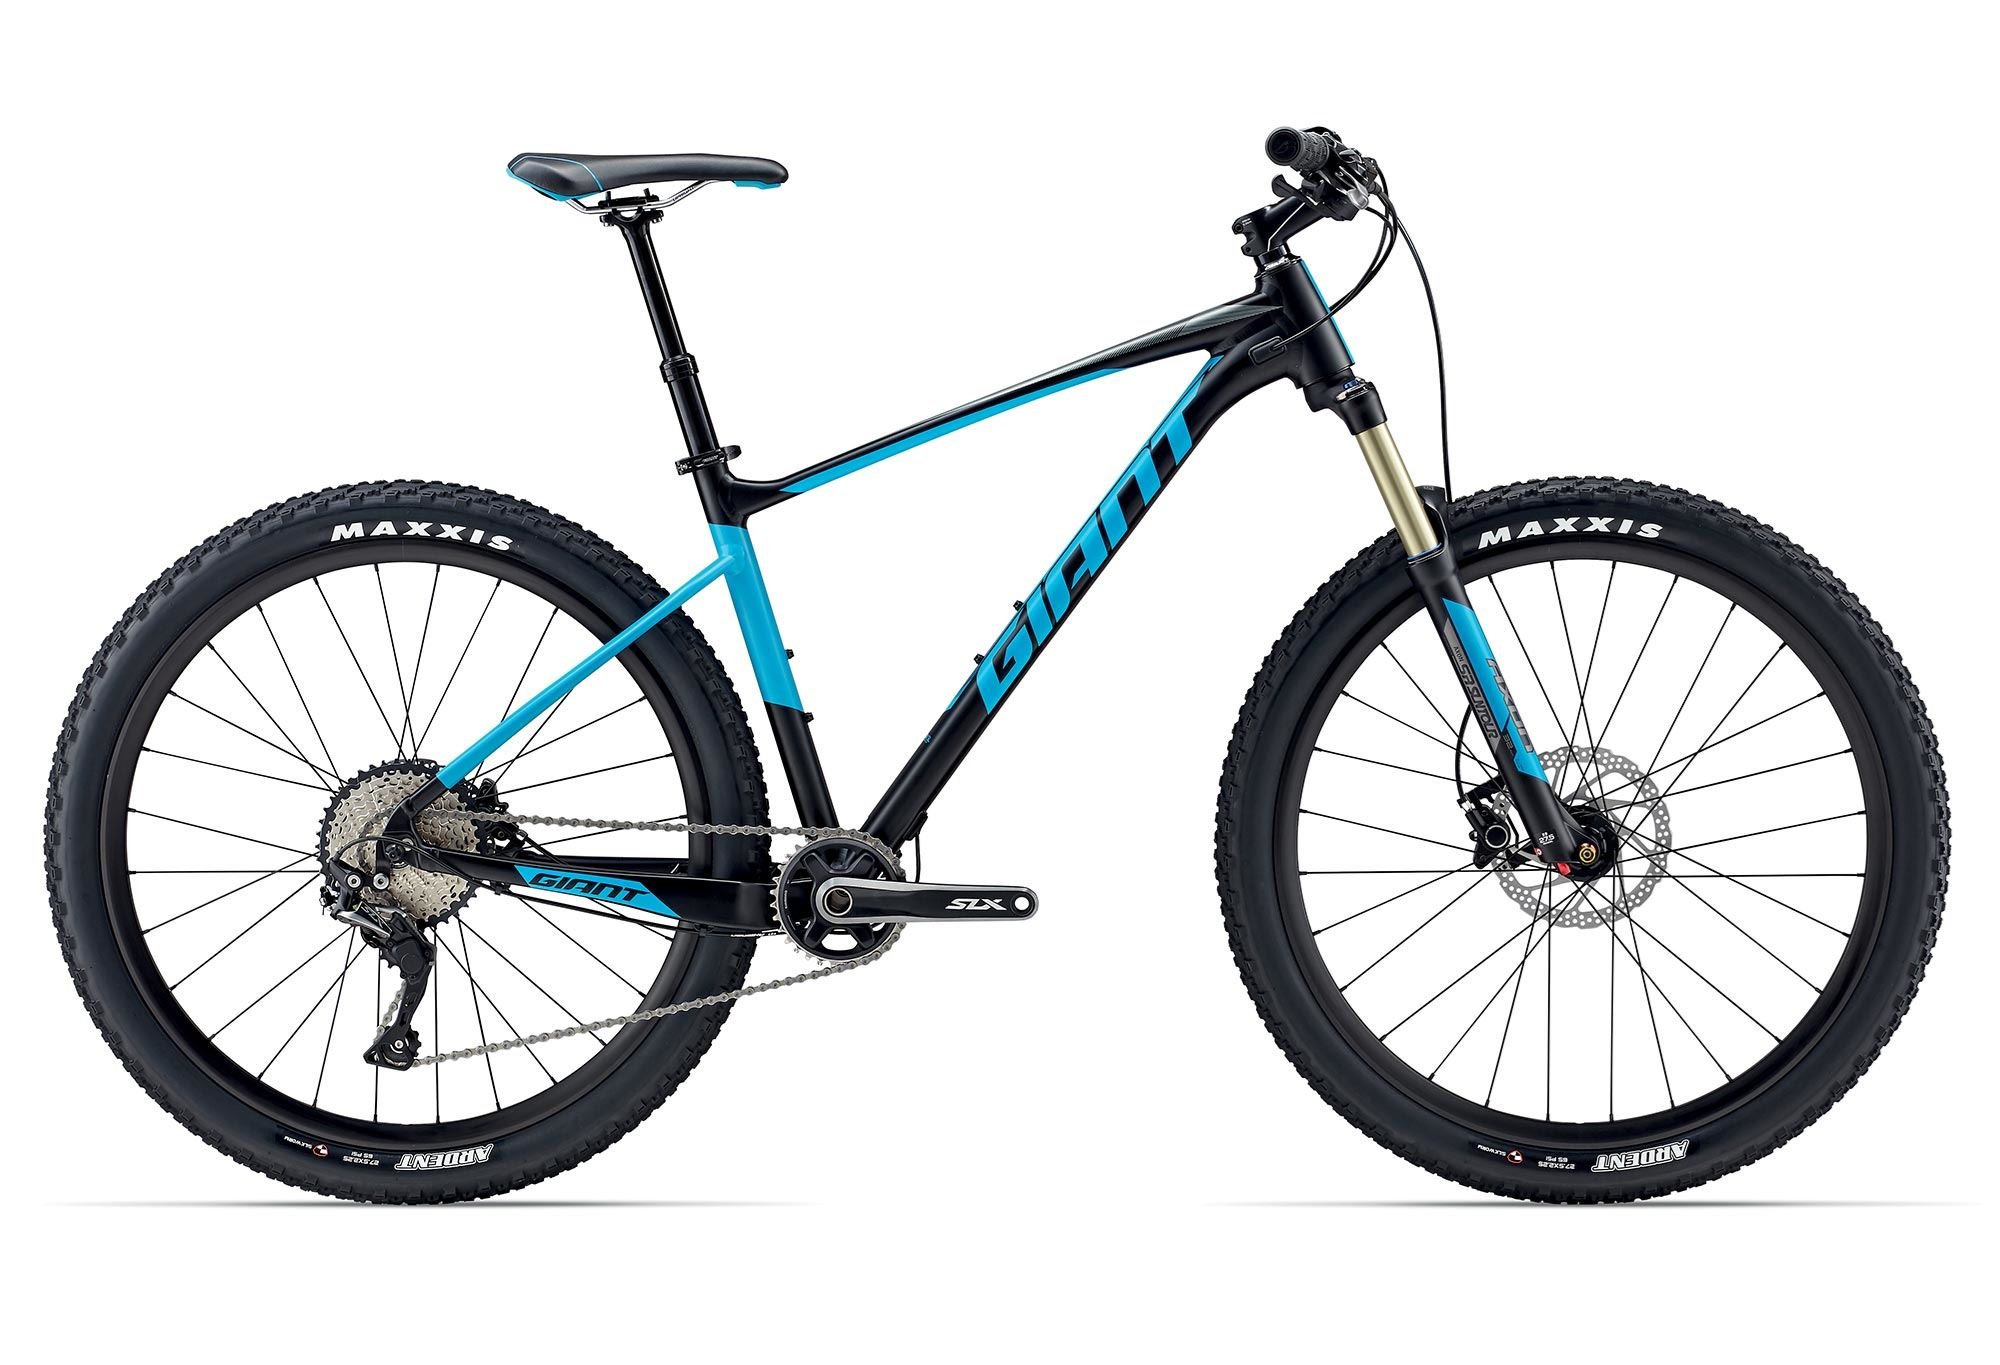
\includegraphics[width=7cm]{../images/2017_GIANT_FATHOM_1.jpg}
		\end{minipage}\hfill
		\begin{minipage}{0.45\textwidth}
			\centering
			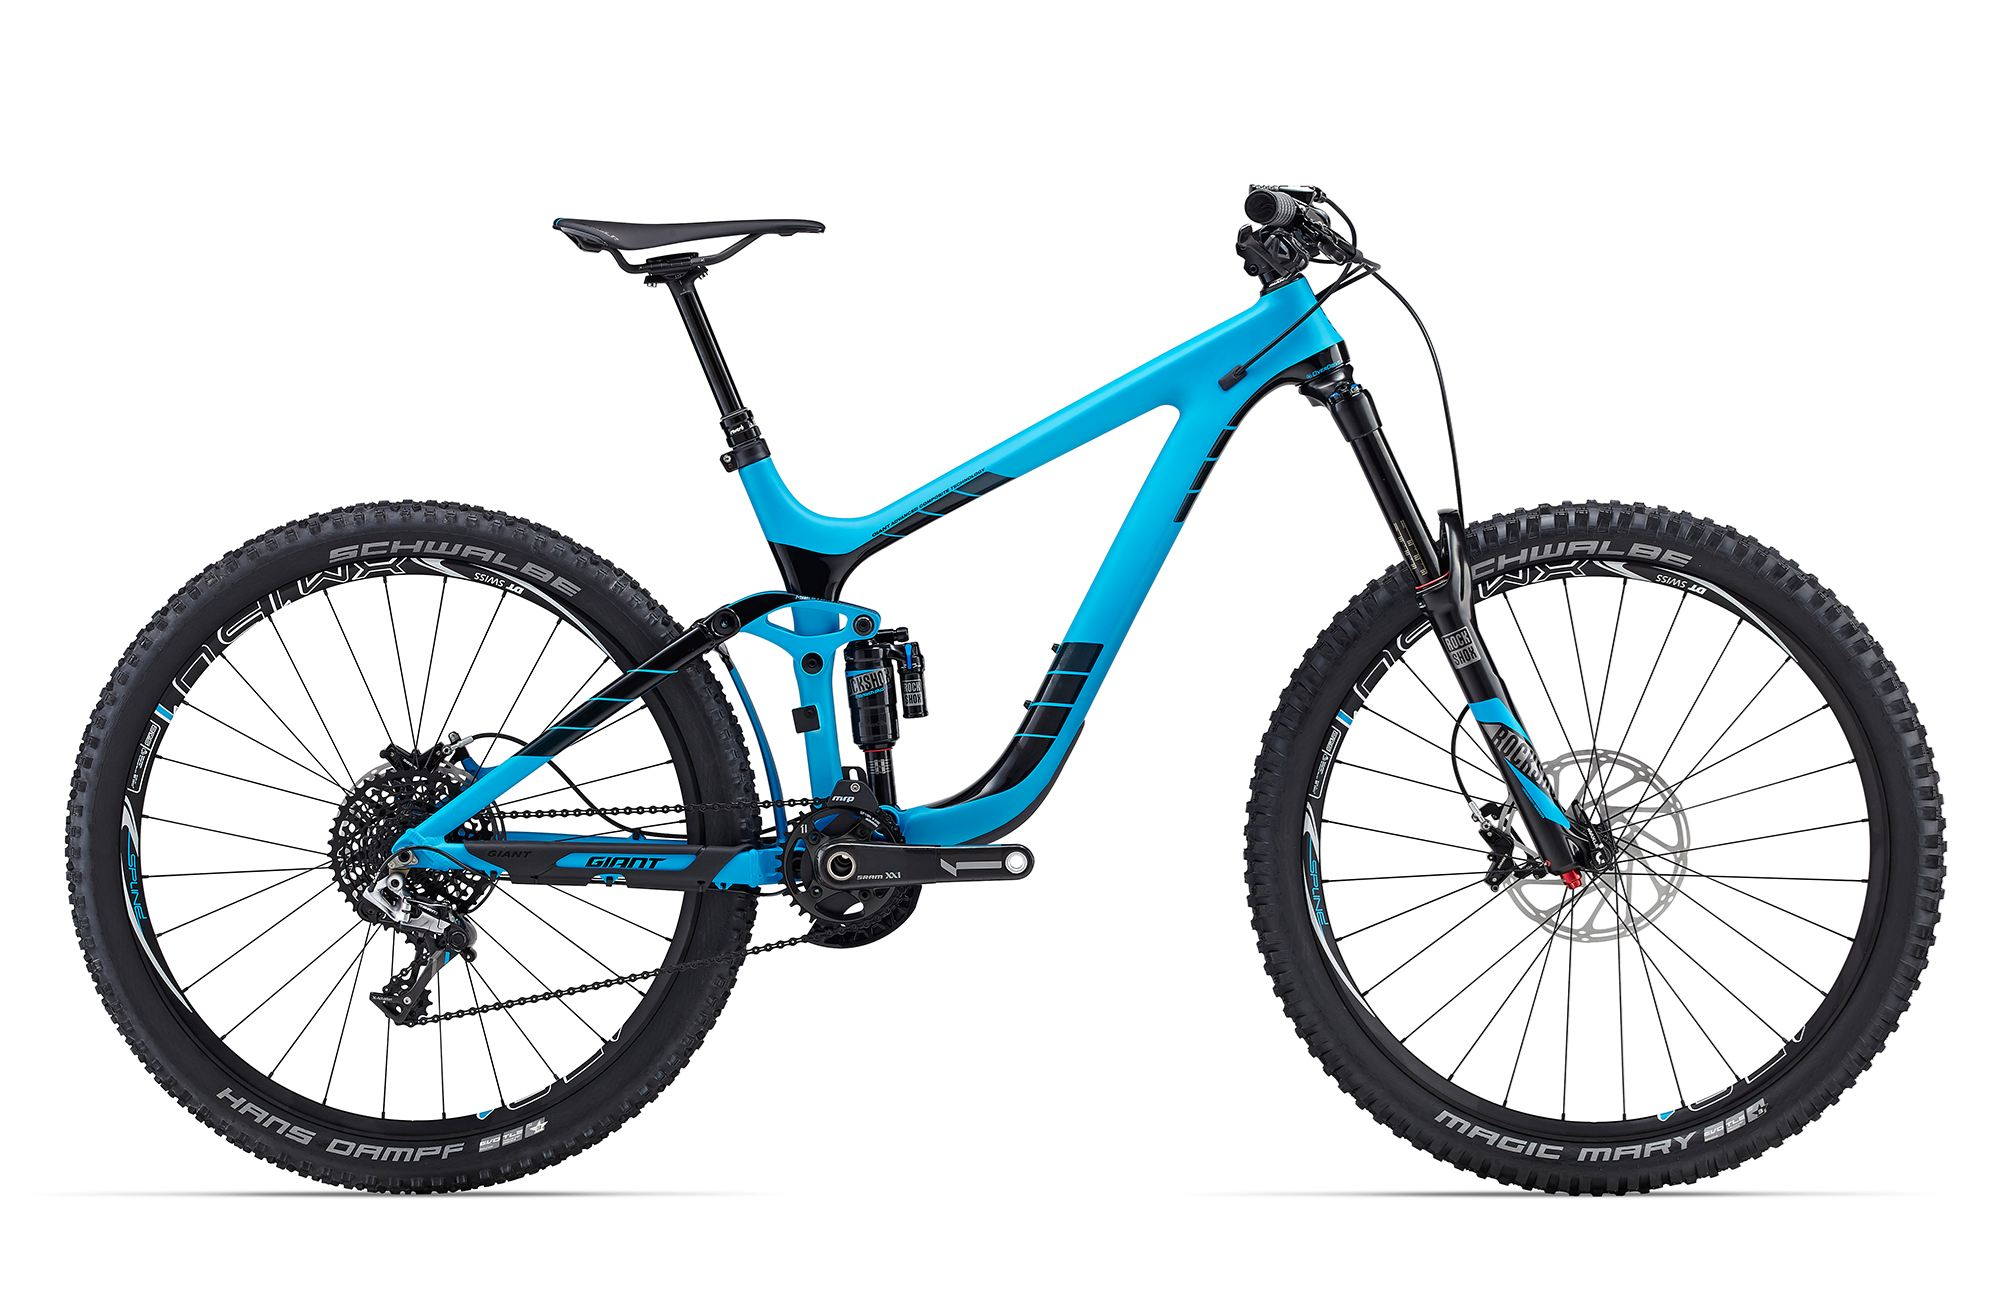
\includegraphics[width=7cm]{../images/2016_Giant_Reign_Advanced_275_0.jpg}
		\end{minipage}
		\caption[Hardtail and full suspension mountain bikes]{Hardtail and full suspension mountain bikes \citep{giantfathom,giantreign}}
		\label{fig:fsandht}
	\end{figure}
	\\
	It has been proven that using a FS bike as opposed to a HT gives the rider a measurable performance advantage \citep{fullsusperf}. However, if the suspension fork and/or rear shock have not been correctly configured it can be detrimental to the rider’s performance and potentially lead to injury. For example, if a \gls{shock} has too little \gls{rebounddamping} applied and the rider goes off a jump, the excessive speed at which the	rear of the bike extends can create forwards rotation, causing the rider to go over the handlebars of the bike. However many enthusiasts lack the specialist knowledge required to optimize the setup of their bike’s suspension units and as a consequence compromise their performance and riding experience.
	\\\\
	Additionally, an incorrect suspension setup can cause excessive wear and tear on the	bike’s frame and components. For instance, suspension which is set too soft will cause “bottoming out” where the unit reaches the end of its available range so that excess forces are transferred to the frame. This causes stress and potentially dramatic fracture that could result in injury. Conversely, suspension that is set too hard forces energy, that would normally be absorbed, into the wheels resulting in denting and warping of the rims.
	\\\\
	Many bicycle retailers will configure the suspension of a newly purchased mountain bike for the customer at the time of collection. Most of the time this will be enough to avoid incident but as the customer is unlikely to be wearing weighty protection equipment and accessories such as helmet, body armour and hydration pack, this initial setup is rarely accurate. Furthermore, with some manufacturers choosing direct sales over
	supplying to local retailers \citep{roseonline,ytonline}, even this rudimentary setup can be omitted altogether.
	\\\\
	Since the birth of the modern smartphone in 2007, brought about by the first generation Apple® iPhone® and introduction of the Android™ mobile operating system, the use of mobile computing in everyday life has grown rapidly. Google™ stated that there were approximately 1.4 billion active Android users worldwide in 2015 \citep{androidusers}.
	\\\\
	The introduction of activity tracking devices and mobile applications such as FitBit \citep{fitbit} and Strava \citep{strava} and their growing popularity \citep{apppopularity} shows that many individuals like to use their smartphones to aid or augment their performance and enjoyment of their chosen hobby or sport. On the back of this increase, a number of companies have launched small devices \citep{sussmybike, shockwiztrademark} and mobile applications \citep{foxird} designed to help riders set up and fine tune their own suspension, either at home or while out on a ride. Each of the devices produced cost more than £100 and require the suspension to have an initial setup in place and the only mobile application capable of producing an initial setup is tied to a single suspension manufacturer.
\subsection{Aims and Objectives}\label{sec:aims_and_objectives}
	The aim of this project is to create a prototype application capable of providing the user with a suggested suspension setup using image analysis techniques. This will be achieved by meeting the following objectives:
	\begin{itemize}
		\item Complete a literature review of mountain bike suspension and image analysis techniques including how image analysis is currently used in sports science
		\item Implement the prototype application using identified and researched methods
		\item Evaluate the success and appropriateness of the produced application
		\item Present conclusions about the project's successes and downfalls
	\end{itemize}
\subsection{Dissertation Structure}
	This dissertation will document the project by taking the following structure:
	\begin{itemize}
		\item[\bfseries \ref{sec:introduction}] {\bfseries Introduction} - Outlines the context of the project and states the major aims and objectives
		\item[\bfseries \ref{sec:lit_review}]{\bfseries Literature Review} - Presents a literature review to further describe the project context and provide information on mountain bike suspension concepts and image analysis techniques
		\item[\bfseries \ref{sec:methodology}] {\bfseries Methodology} - Discusses the methodologies available which could be used to complete the project and their advantages
		\item[\bfseries \ref{sec:results}] {\bfseries Results} - Describes the outcome of the project including any deviations from the plan, the operation of the application, and a critical evaluation of the application
		\item[\bfseries \ref{sec:conclusion}] {\bfseries Conclusion} - Presents conclusions and learnings from completion of the project including potential future work and a self appraisal
	\end{itemize}
	
	\section{Literature Review}
	The purpose of this section is to introduce the concepts of mountain bike suspension setup and indicate why this may be difficult for a less knowledgeable individuals. It will then continue to identify and explain common image analysis techniques and how they may be applied to mountain bike suspension setup.
		\subsection{Mountain Bike Suspension Concepts}
		The purpose of suspension on a mountain bike is to absorb the energy created from riding over features such as bumps and rough terrain encountered along a trail, improving comfort for the rider and allowing them to go faster by maintaining better contact between the tires and the ground. This requires the use of a spring and damper, collectively known as a shock absorber, which allows the wheel to move away from the feature on contact and make a controlled return once it has been passed.
	\subsubsection{Travel and Stroke}
		\Gls{travel} is the distance which the bike’s fork or frame allow the wheel to move in an upward direction while \gls{stroke} is the distance that the shock absorber can compress before it bottoms out. \Gls{travel} is measured in millimetres or inches and can range from 80mm to 210mm or 4in to 9in. Bikes designed for different disciplines require differing amounts of travel with those designed for cross-country riding typically requiring less travel than those designed for more aggressive disciplines such as downhill racing having more. See Table \ref{tab:travel} for typical specifications.
		\begin{table}[h!]
		\centering
		\caption{Table of common suspension \glspl{travel} and intended disciplines}
		\label{tab:travel}
		\begin{tabular}{|c|cccc|}
			\hline
			Travel (mm)&Cross Country&Trail&Enduro&Downhill\\
			\hline
			80&\cellcolor[gray]{0.5}&&&
			\\
			100&\cellcolor[gray]{0.5}&&&
			\\
			120&\cellcolor[gray]{0.5}&\cellcolor[gray]{0.5}&&
			\\
			140&&\cellcolor[gray]{0.5}&\cellcolor[gray]{0.5}&
			\\
			160&&&\cellcolor[gray]{0.5}&
			\\
			180&&&\cellcolor[gray]{0.5}&\cellcolor[gray]{0.5}
			\\
			+200&&&&\cellcolor[gray]{0.5}\\
			\hline
		\end{tabular}
	\end{table}
	\begin{figure}[h!]
		\centering
		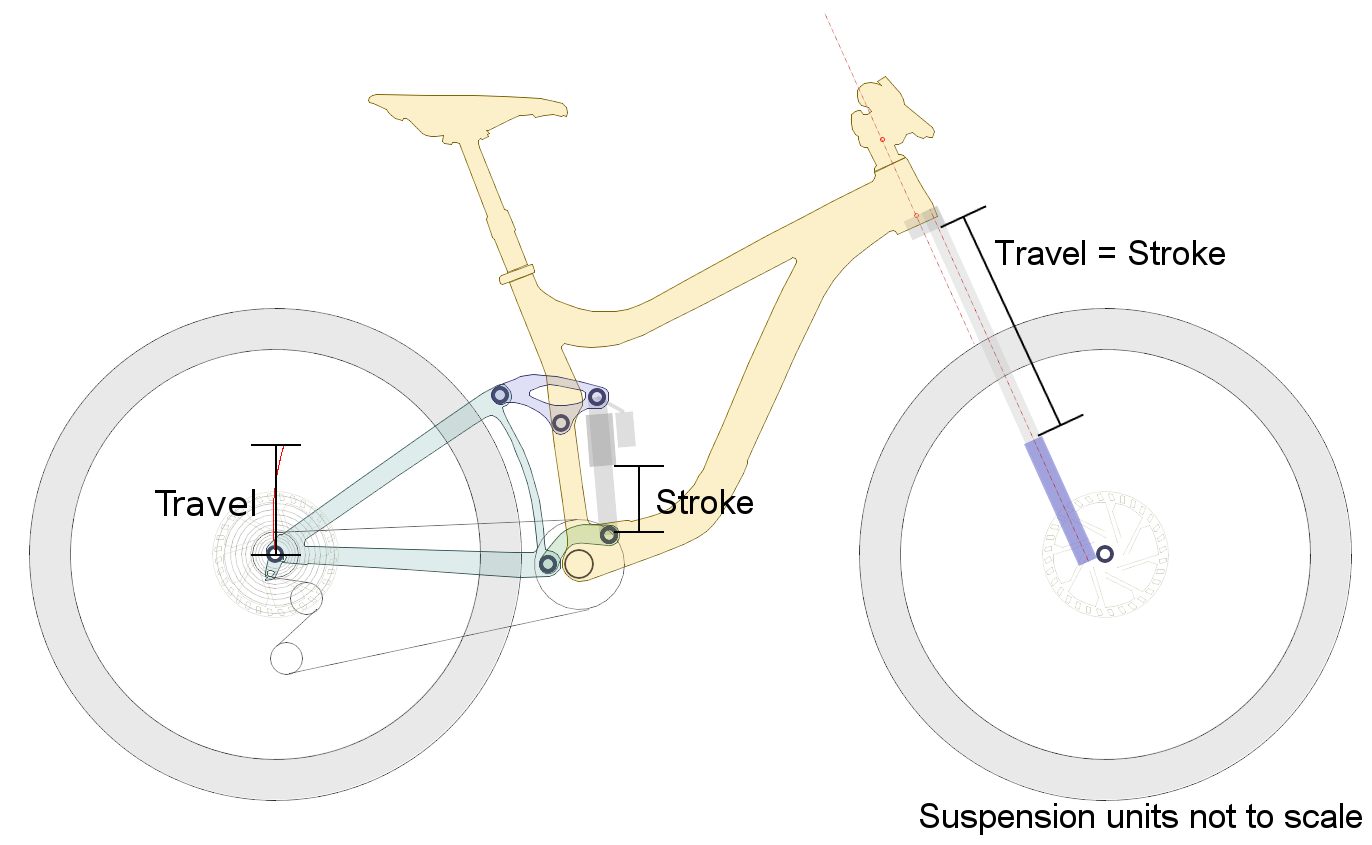
\includegraphics[width=12cm]{../images/reignschpath.PNG}
		\caption[Diagram showing travel and stroke on a full suspension bike]{Diagram showing 
			travel and stroke on a full suspension bike\footnotemark}
		\label{fig:travelvsstroke}
	\end{figure}
	\subsubsection{Front Suspension}
		Front suspension commonly employs a linear telescoping shock absorber, known as a \gls{fork} due to it's dual sided construction. On nearly all suspension \glspl{fork} the \gls{stroke} is 1:1 with the potential travel of the wheel. Front suspension is found on 
		all \gls{fs} and \gls{ht} bikes.
	\subsubsection{Rear Suspension}\label{sec:lit_review_rear_suspension}
		Rear suspension uses a shock absorber that is much shorter than a fork so it cannot operate on a 1:1 ratio and still allow the desired travel. Full suspension frames incorporate one or more pivot points and linkages which allow the wheel to move and act as multipliers for the suspension. Rear ratios are expressed as n:1 where n is the average distance the rear wheel moves for every 1mm the shock compresses throughout its stroke; the leverage ratio changing constantly across the compression cycle.
		\\\\
		The difference between front and rear stroke and travel can be seen in Figure \ref{fig:travelvsstroke} noting the separation of rear wheel travel from the stroke of the shock absorber. Although manufacturers design their rear suspension differently, the rear wheel always rotates around the main pivot, (or in some cases a virtual pivot), as opposed to moving linearly as front forks do. As a result, the frame behaves differently through its travel, depending on the number and location of pivot points and the type of shock that it is being used. 
		\\\\
		Because of this the average ratio is normally dismissed in favour of a leverage curve that plots the ratio n:1 throughout the compression cycle. Figure \ref{fig:3_bike_lev_ratio} shows the leverage curves of three modern suspension designs. Each of these designs has between 150mm and 170mm of travel and uses the 27.5 inch wheel size. However, it is evident that varying the location of pivot points produces suspension with drastically different characteristics.
		\begin{figure}[h!]
			\centering
			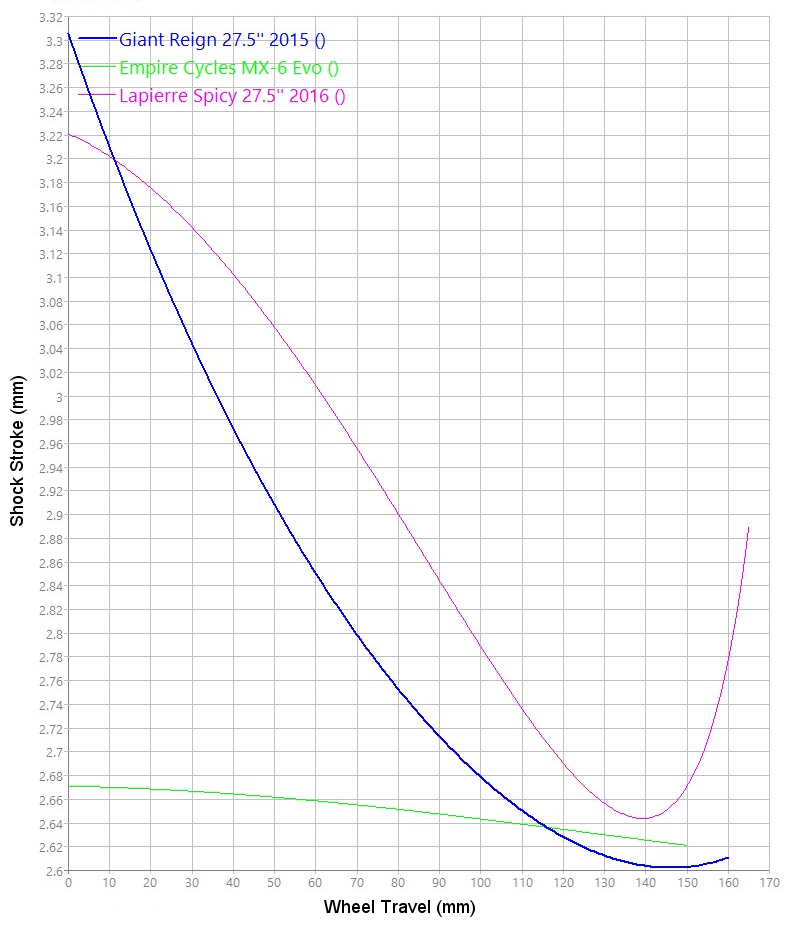
\includegraphics[width=10cm]{../images/3_bike_lev_ratio.jpg}
			\caption{Leverage curves of three modern suspension designs}
			\label{fig:3_bike_lev_ratio}
		\end{figure}
		\\
		The Virtual Pivot Point (VPP) design of the Giant Reign (shown blue) has an initial falling rate, meaning the shock can be compressed easily, but slows down and even rises slightly towards the end of its travel as seen in Figure \ref{fig:3_bike_lev_ratio}. This means the suspension will feel soft most of the time but stiffer as compression increases. This is emphasised by the Horst link system of the Lapierre Spicy (shown magenta) where the leverage curve rises significantly towards the end of its travel.In contrast, the curve of the single pivot Empire MX-6 Evo (shown green) is effectively linear. This is due to the MX-6 having only one pivot and swinging arm, as opposed to multiple pivots and linkages of the VPP and horst link designs, so there is an almost direct input from the rear wheel to the shock. The physical differences in each of these frames can be seen in Figure \ref{fig:3_bike_diagrams}.
		\begin{figure}[h!]
			\centering
			\begin{subfigure}[t]{0.3\textwidth}
				\centering
				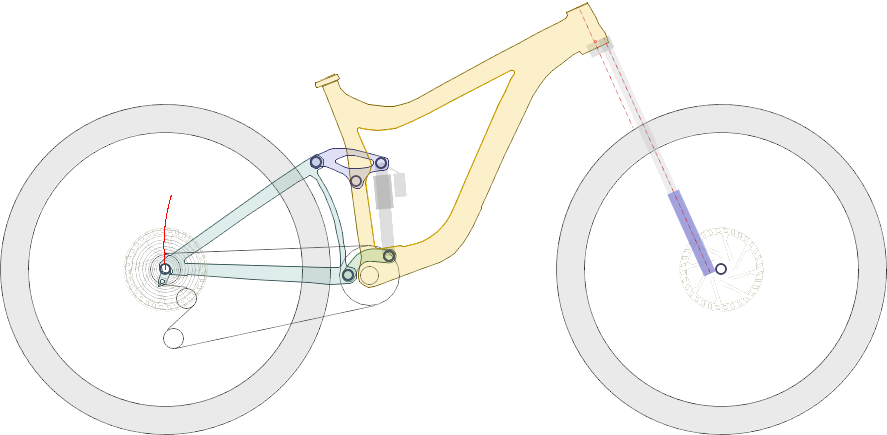
\includegraphics[width=\textwidth]{../images/3_bikes/giant.png}
				\subcaption{Giant Reign}
			\end{subfigure}
			\begin{subfigure}[t]{0.3\textwidth}
				\centering
				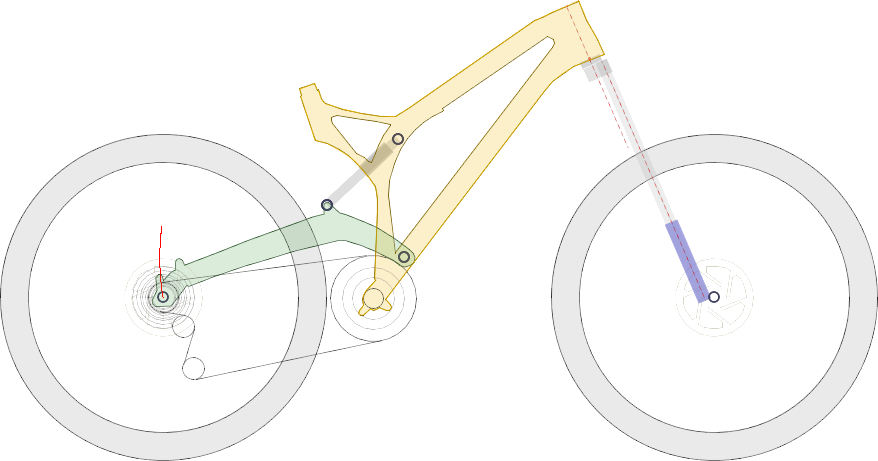
\includegraphics[width=\textwidth]{../images/3_bikes/empire.png}
				\subcaption{Empire MX6 Evo}
			\end{subfigure}
			\begin{subfigure}[t]{0.3\textwidth}
				\centering
				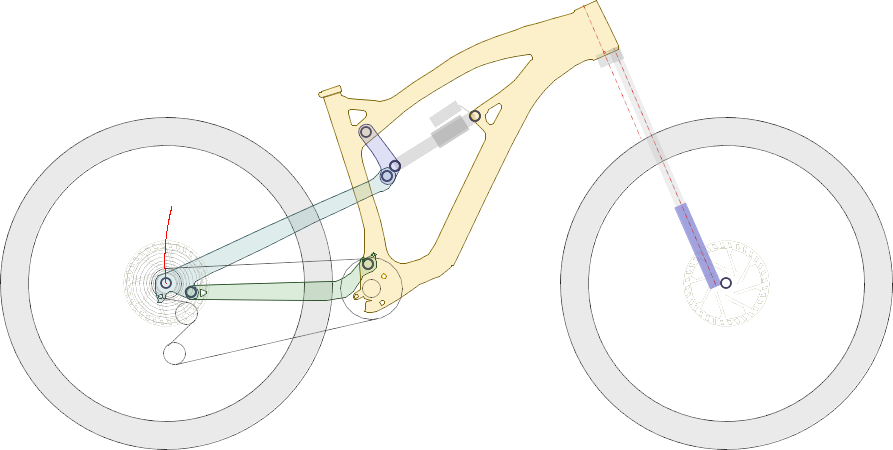
\includegraphics[width=\textwidth]{../images/3_bikes/lapierre.png}
				\subcaption{Lapierre Spicy}
			\end{subfigure}
			\caption{Full suspension frame comparison}
			\label{fig:3_bike_diagrams}
		\end{figure}
		\\
		For this project two bikes will be used for development and testing of the application. The first is a 2015 Giant Reign, shown on figure 3 in blue, as it will be constantly available throughout the project. The frame uses Giant’s Maestro™suspension system which is a variation of VPP. Like all VPP systems Maestro uses two links, an upper and lower, to create a virtual main pivot point, however unlike other VPP systems, Maestro creates its virtual pivot as close to the rear of the frame as possible As shown by the red circle in Figure \ref{fig:maestro}. The second will be a 2011 Orange 5 which has the same suspension design as the Empire MX6 Evo in Figure \ref{fig:3_bike_lev_ratio}. This bike was selected as it has a completely different design to the Giant Reign and will also be easily accessible throughout the project. 
		\begin{figure}[h!]
			\centering
			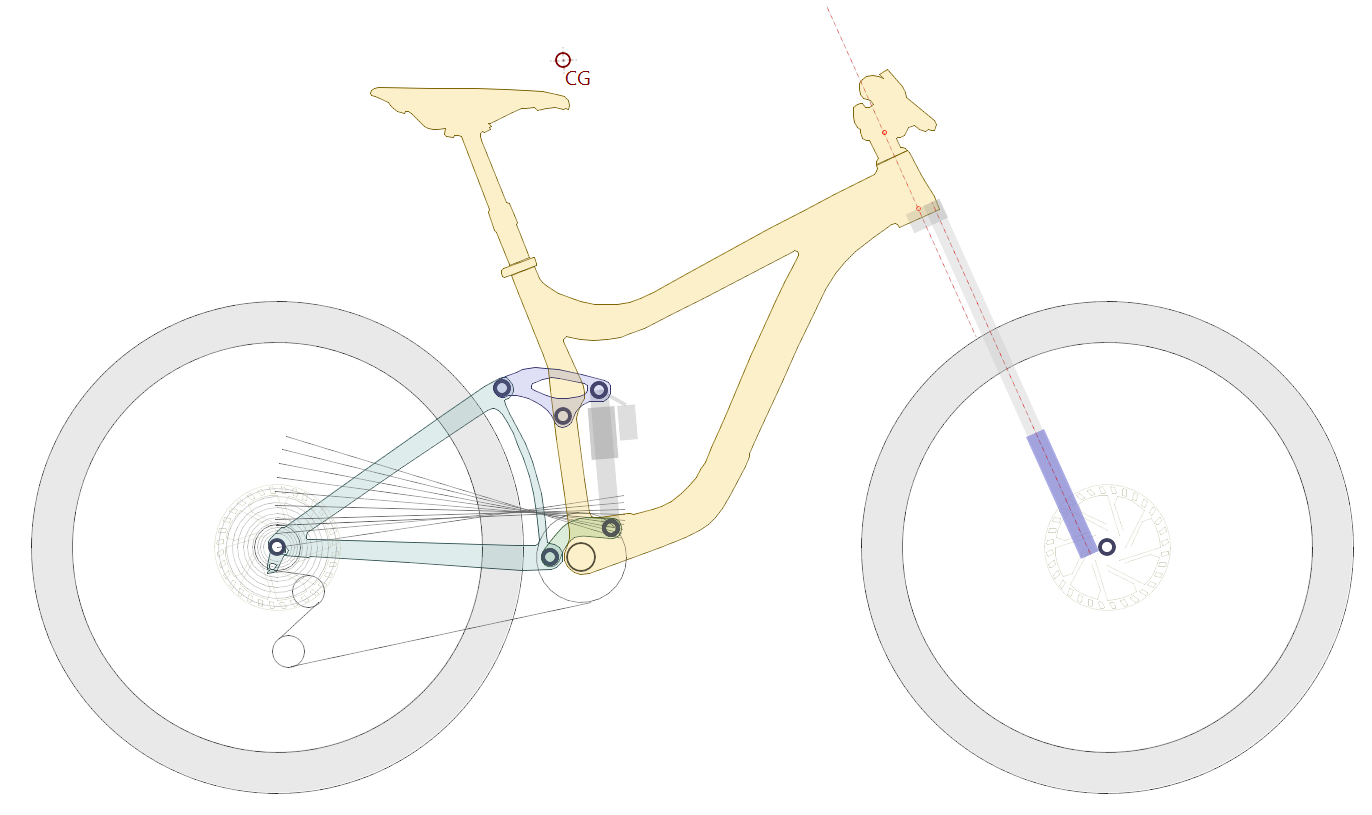
\includegraphics[width=12cm]{../images/reignsch.PNG}
			\caption{Maestro suspension}
			\label{fig:maestro}
		\end{figure}
		\\
		Although rear suspension designs are complex, neither the average rider nor professionals, such as mechanics, working in the industry necessarily need this specialist knowledge. Leverage curves are predominantly used by designers to determine how a particular suspension unit will behave when researching and designing new frames \citep{creek2016curves}. Though having an understanding of leverage curves will help the individual rider to fine tune their suspensions settings described in the following sections themselves, the majority will take little interest in the differences between a single pivot and VPP design, choosing a simpler ”set and forget” approach to their suspension. 
		\\\\
		In the context of this project and the intended user for the application, this begs the question of how much information should be provided to the user? Modern human /computer interaction principles aim toward providing information to the user which is relevant and necessary in context \citep{shneiderman2010designing}. Presenting the user with a leverage curve which may require extensive interpretation before they understand the implications within the limitations of a mobile application may prove detrimental to the user experience. For an application which is intended to remove the difficulties of suspension setup and allow for quick and easy production of a basic setup, providing a single sag setting would be preferable over a plethora of of technical data.	
	\subsubsection{Sag} \label{sec:sag}
		\todo{review section adding detail on setup method}
		Sag is the amount that the suspension sits into its travel when the rider is in a neutral position, described in Figure \ref{fig:sag}. It is required so that the suspension has travel available to extend as well as just compress and is calculated using the rider’s weight, available travel, and intended riding style.
		\\\\
		The amount of sag depends on the stiffness of the suspension unit which can be adjusted by changing the air pressure of an air spring or replacing the spring and adjusting the preload of a traditional coil shock. Depending on discipline and the	amount of travel the bike has, sag can vary between 15\% and 40\% of the available travel though it is typically set at between 25\% and 35\% for the average rider with greater variances only encountered in competition.
		\begin{figure}[h!]
			\centering
			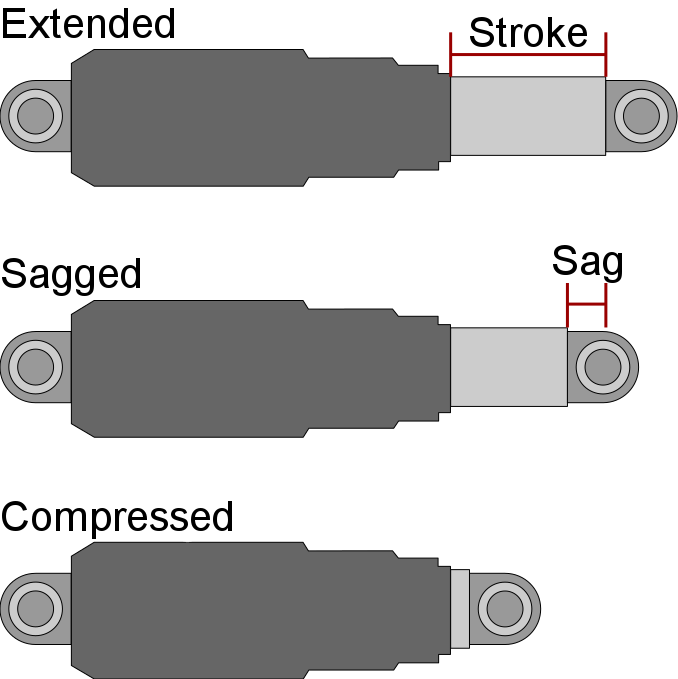
\includegraphics[scale=0.5]{../images/sag_diagram.png}
			\caption{Diagram of shock states indicating sag}
			\label{fig:sag}
		\end{figure}
		\\
		Sag is set by first calculating the distance that the shock should sit into its travel by producing the desired percentage of the shocks stroke. For an air shock the manufacturers recommended pressure is then pumped into the shock and the rider weights the bike. On each air shock there is a marker o-ring which is pushed down the shock shaft when the shock is compressed. The position this o-ring ends at can be measured and the shock pressure adjusted accordingly until it sits at the target measurement. 
	\subsubsection{Damping}
		In a spring and mass system, when the spring is elongated it will exert a returning force on the mass which, according to Hooke's law \citep{rychlewski1984hooke}, is directly proportionate to the distance which the spring has been pulled. In suspension this force is explained as two separate forces. If an individual were to push down on mountain bike suspension they would feel a resistance, this is known as compression, and when they let go the suspension will return to its neutral state, this is rebound. Both of these can be controlled which is known as damping.
		\\\\
		Suspension damping works by forcing oil within the shock absorber through a series of holes in the absorber’s damping circuit. Reducing the size or number	of holes increases resistance, reducing the speed at which the oil flows through the circuit to increase the damping effect by making compression and rebound slower.
	\paragraph{Compression Damping} 
		This is applied while the shock absorber is being compressed to control the effort required to do so. Increasing damping forces the wheel to remain in contact with the ground which makes the suspension feel stiffer. However too much compression damping can make the suspension overly stiff so it does not effectively absorb the impact of bumps and rough terrain. Conversely, too little compression damping can cause the suspension to ”blow through” all of the available travel prematurely with nothing left to soak up impact when it is most required. 
	\paragraph{Rebound Damping}
		This is used to control the speed at which the shock absorber recovers to its normal riding position after compression. An optimal setting will allow the suspension to track the ground, quickly and smoothly returning to the correct position after a bump or hole is passed. 
		\\\\
		Too much rebound damping causes the suspension unit to recover slowly and sometimes “pack down” meaning the shock absorber remains compressed for too long leaving the rider fully exposed to the next impact. Too little rebound damping can cause the suspension to “buck” the rider, like a horse, and potentially cause an accident.
	\paragraph{High and Low Speed Damping} 
		The ways of adjusting compression and rebound damping differ by manufacturer and model with better specified bikes having two adjustable speeds for each damping circuit giving four damping settings. High speed adjustments are used in high G-force situations such as riding large jumps or drops where compression needs to be set softer to absorb impacts and rebound set slower so the rider has time to recover without the equilibrium of the bike being upset.
		\\\\
		Low speed damping set ups are used against lower G-force movements such as rider weight shifts or long, slow compressions. Optimally compression is set stiffer as this type of feature can use a lot of travel and rebound damping set faster to deal with multiple features in quick succession.
	\subsubsection{Optimal Setup}
		Although setups will vary between rider, suspension system and discipline, there are some key principles that all riders should aim to achieve. Sag should be set to an appropriate measurement by adjusting the air pressure on air shocks or spring rating on coil shocks. Compression damping should feel soft and soak up bumps efficiently without excessive bottoming out. Rebound damping should be set to return as fast as possible without bucking the rider, which is normally somewhere in the middle of the two setting available with a slight bias towards the faster option.
		\\\\
		Attaining this optimal setup can be difficult for both beginners and intermediate riders as they lack experience and in-depth knowledge of suspension units and may not know how different frames react while being ridden. Knowing which measurements to make and the calculations required to correctly configure sag, compression and rebound settings are typically beyond the capabilities of this level of rider unless they have been previously trained by a professional or investigated the topic in detail for themselves.
	\subsection{Image Analysis}
	\gls{ia} is the use of various techniques such as pattern recognition, geometry calculations, and signal processing to extract information from digital images for later use. Image processing however is the application of various processes on an image to change or improve the way it looks. The processing stage normally comes before the analysis stage in an effort to simplify the analysis processes and improve their success.
	\begin{figure}[h!]
		\centering
		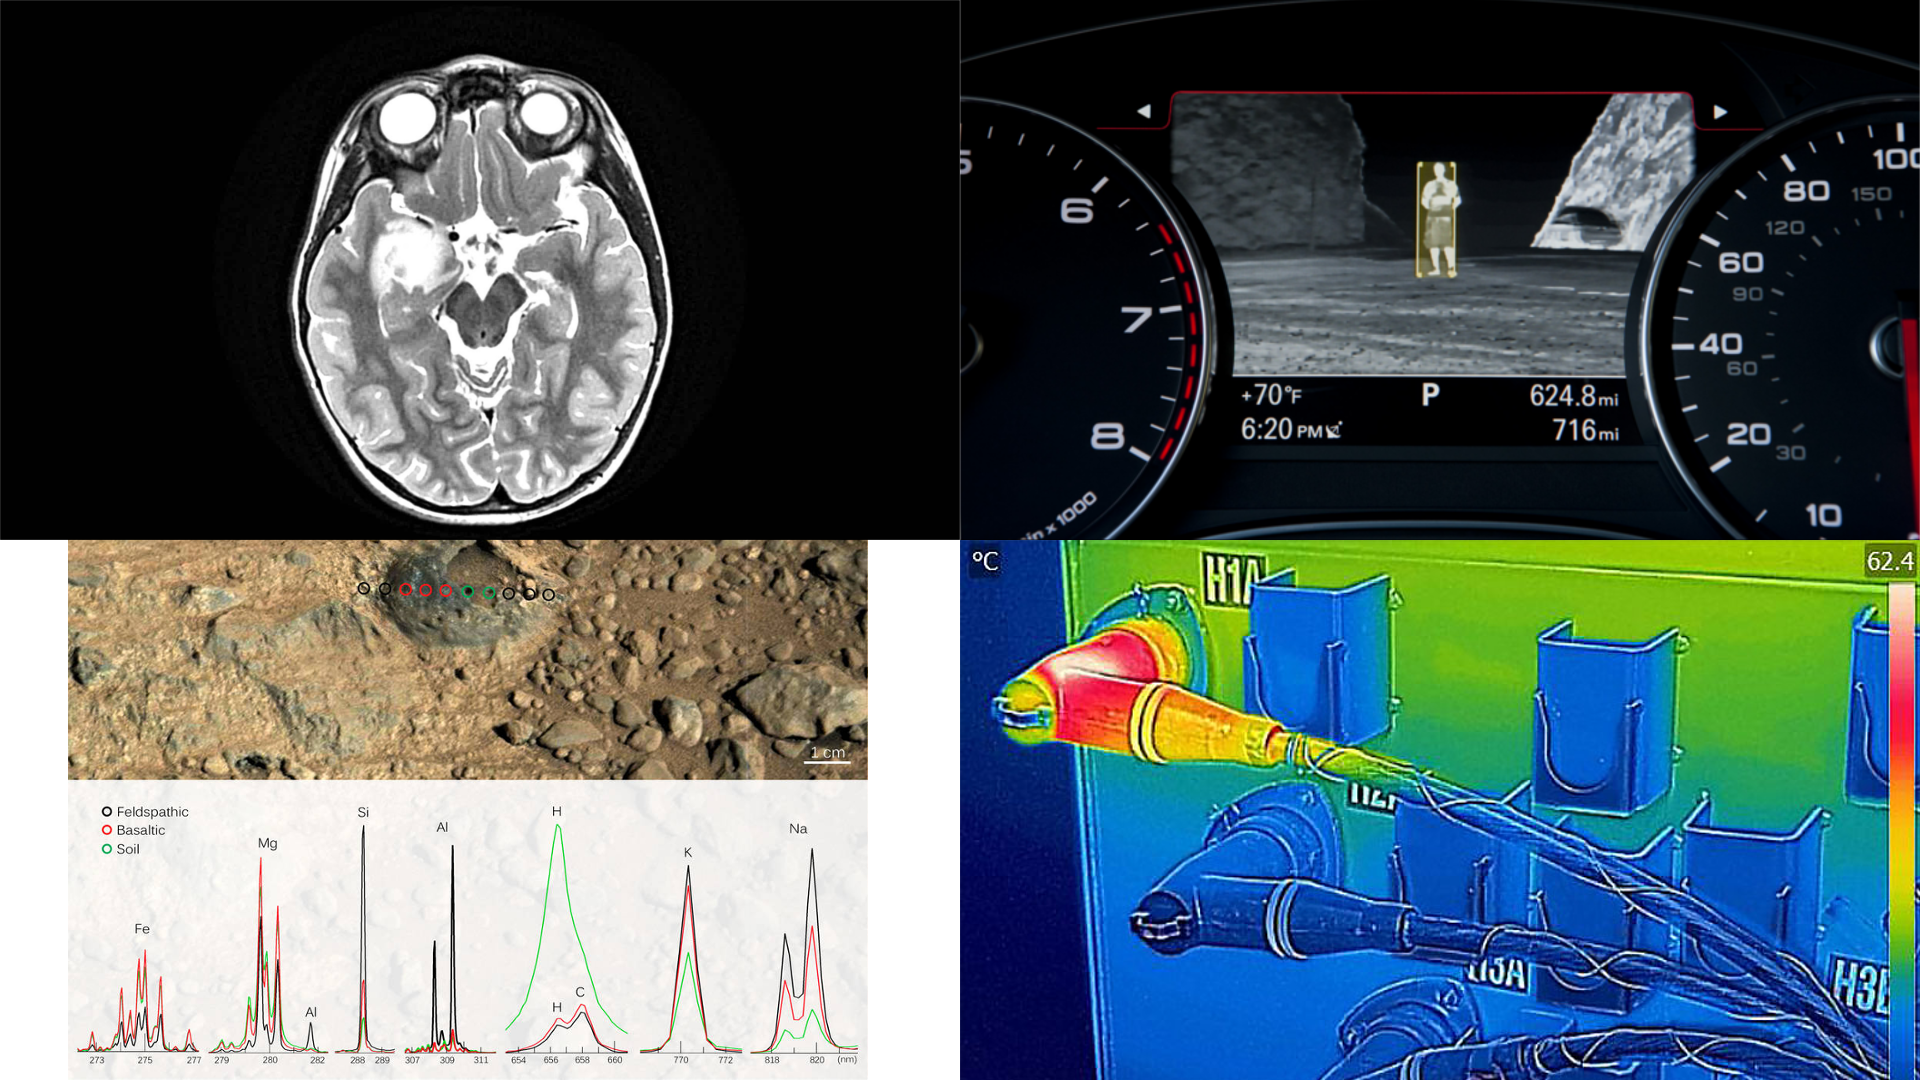
\includegraphics[width=15cm]{../images/4panel.png}
		\caption{Uses of image analysis, from top left clockwise: An MRI brain scan, automotive night vision with pedestrian recognition, infrared image taken with a smartphone, chemical rock analysis from mars}			
		\label{fig:curiosity}
	\end{figure}
	\subsubsection{Usages}
	Image processing and analysis has been applied to multiple areas with its value and effectiveness rapidly improving alongside camera technology and computing power. These applications range from recognising faces in social media uploads \citep{zuckerberg2011tagging} to the utilisation of satellite imagery to tracking the changing shape of coastlines \citep{costalimagery}.
	\paragraph{Medical}
	Arguably one of the most important uses of \gls{ia}, advances in medical imaging have reduced costs in healthcare, diagnosis time, recovery time, and improved the ability to localise and personalise treatments \citep{esfmedical}. Major uses of \gls{ia} in medical applications are the use of Magnetic Resonance Imaging (MRI) and Computerised Topography Scanning (CT Scan) to create detailed images of the human body and identify illness before some symptoms arise.
	\paragraph{Transport}
	Image analysis has been included in the consumer automotive market on various models since 2004 when Honda introduced an thermographic night vision camera with pedestrian detection on the Legend  \citep{hondanightvision}. Since this initial introduction many vehicle manufacturers have included image analysis and recognition features as options such as speed limit sign recognition, lane departure warning systems, and automatic braking systems based on hazard recognition.
	\paragraph{Engineering}
	The use of image analysis in engineering has pushed to create more stable and efficient structures by looking at the materials used in their construction \citep{concreteanalysis} and monitoring their stresses and potential weak areas \citep{bridgecables}. Using image analysis by engineers on site has become more common with the advances in mobile computing and some manufacturers aiming their products at an engineering demographic with features like improved durability and built in infrared imaging \citep{catphone}.
	\paragraph{Space}
	While some industries make use of satellite imagery to monitor changes on our own planet, agencies such as NASA and ESA make use of image analysis to look at planets and other celestial bodies. The Martian rover, Curiosity, uses multiple cameras for navigation, hazard avoidance, and scientific imaging the products of which are streamed back to Earth for analysis. Major uses for the various types of images returned include identification of geological formations and compositions \citep{curiositysand, curiositygravel} and chemical location and identification using the "ChemCam" \citep{curiosityhydrogen}.
	\subsubsection{Image Analysis Techniques}
	There are multiple techniques which can be applied to imagery to extract information which include detection of edges or objects and using known data to take measurements. These methods tend to compare data from neighbouring pixels to spot differences which can indicate features.
	\paragraph{Edge Detection}
	This is the application of mathematical algorithms to locate and highlight the edges of features in an image. There are multiple algorithms which can be used for edge detection including Sobel, Roberts, Canny, and fuzzy logic though all utilise the concept of comparing side by side pixel data to find "steps" from one brightness to another.
	\begin{table}[h!]
		\centering
		\caption{Table of pixel data showing an edge}
		\label{tab:edgePixels}
		\begin{tabular}{|c|c|c|c|c|c|c|}
			\hline
			5&7&6&4&152&148&149\\
			\hline
			\cellcolor[HTML]{0D0D0D}&
			\cellcolor[HTML]{121212}&
			\cellcolor[HTML]{0F0F0F}&
			\cellcolor[HTML]{0a0a0a}&
			\cellcolor[HTML]{989898}&
			\cellcolor[HTML]{949494}&
			\cellcolor[HTML]{959595}\\
			\hline
		\end{tabular}
	\end{table}\\
	Table \ref{tab:edgePixels} represents possible pixel values of an edge indicated by the large difference between 4 and 152. The applied algorithm will pick up on this discrepancy and in will be indicated on the resulting image. A common application for edge detection is text recognition such as in automatic number plate recognition (ANPR) \citep{anpr} as the process can remove unwanted background data and highlight the block shapes of the number plate.
	\begin{figure}[h!]
		\centering
		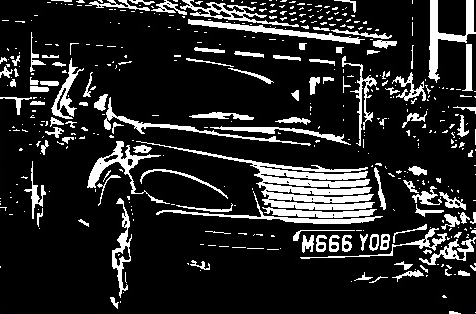
\includegraphics[width=10cm]{../images/anpr.jpg}
		\caption{Edge detection applied to an image for number plate recognition}
		\label{fig:anpr}
	\end{figure} 
	\paragraph{Object Detection}
	Much like edge detection, object detection is used to pick out features in images, the 
	difference being that object is a more abstracted term than edge and could mean anything from 
	faces to signs to company logos. A common technique is Binary Large OBject (BLOB) analysis 
	which is two techniques combined into one application \citep{introtoprocessing}, this includes 
	BLOB extraction which is used to isolate large objects in an image, dismissing small objects as 
	noise, which is then followed by BLOB classification, assigning objects a class based on 
	predetermined parameters.
	\\\\
	Regularly carried out after grayscaling and thresholding an image, BLOB extraction uses a grass-fire algorithm to locate pixels which display a significant difference to the image background and discover the full extent of this region. As all the pixels of each BLOB in a object are known, certain parameters are also known such as size, area, and boundaries. From these parameters, calculations can be carried out to discover the classification of each BLOB, for example with the boundary and area of each BLOB, the circularity can be calculated to locate all the circular objects in an image.
	\begin{equation}
		B_{c}=\frac{B_{p}}{2\sqrt{\pi \times B_{a}}}
	\end{equation}
	\begin{where}
		\item $B_{c}$ is the circularity of the BLOB
		\item $B_{p}$ is the perimeter of the BLOB's bounding box
		\item $B_{a}$ is the area of the BLOB
	\end{where}
	\paragraph{Taking Measurements}
	To measure an object in an image, certain data about the camera and camera's location are 
	required. By using digital imagery the majority of this information is provided as each image 
	contains metadata or EXchangeable Image Format (EXIF) data which includes information such as 
	camera manufacturer, focal length, image size, and location.
	\begin{equation}
		\label{equ:measureobj}
		H_{o} = \Bigg(\frac{f\times\big(\frac{H_{i}}{H_{s}}\big)}{D - f}\Bigg)\times H_{c}
	\end{equation}
	\begin{where}
		\item $f$~~~~is the focal length of the camera lens
		\item $D$~~~is the distance to the object
		\item $H_{o}$~~is the height of the object
		\item $H_{i}$~~is the height of the image in pixels
		\item $H_{s}$~~is the height of the camera sensor
		\item $H_{c}$~~is the height of the camera from the ground
	\end{where}
	\begin{comment}
	\begin{equation}
	\label{equ:measuredist}
		D = \frac{f\times H_{c} \times H_{i}}{H_{o} \times H_{s}}
	\end{equation}
	\begin{where}
		\item $D$~~~is the distance to the object
		\item $f$~~~~is the focal length of the camera lens
		\item $H_{c}$~~is the height of the camera from the ground
		\item $H_{i}$~~is the height of the image in pixels
		\item $H_{o}$~~is the height of the object
		\item $H_{s}$~~is the height of the camera sensor
	\end{where}
	\end{comment}
	\vspace{5mm}
	The process to calculate the height of an object in an image is shown in equation 
	\ref{equ:measureobj}. $f$, $H_{i}$, and $H_{s}$ can be acquired from EXIF 
	data, however $D$ and $H_{c}$ are not collected by the camera and must be measured. When 
	dealing with image analysis this means that this data must have been collected when the image 
	was taken.
	\\\\
	To circumvent the need for this data a reference object of known size can be included in the 
	image, this allows a comparison between the object to be measured and the reference object. The 
	previously mentioned mars rover, Curiosity, carries a United States penny and charts to 
	calibrate its cameras against.
	\begin{figure}[h!]
		\centering
		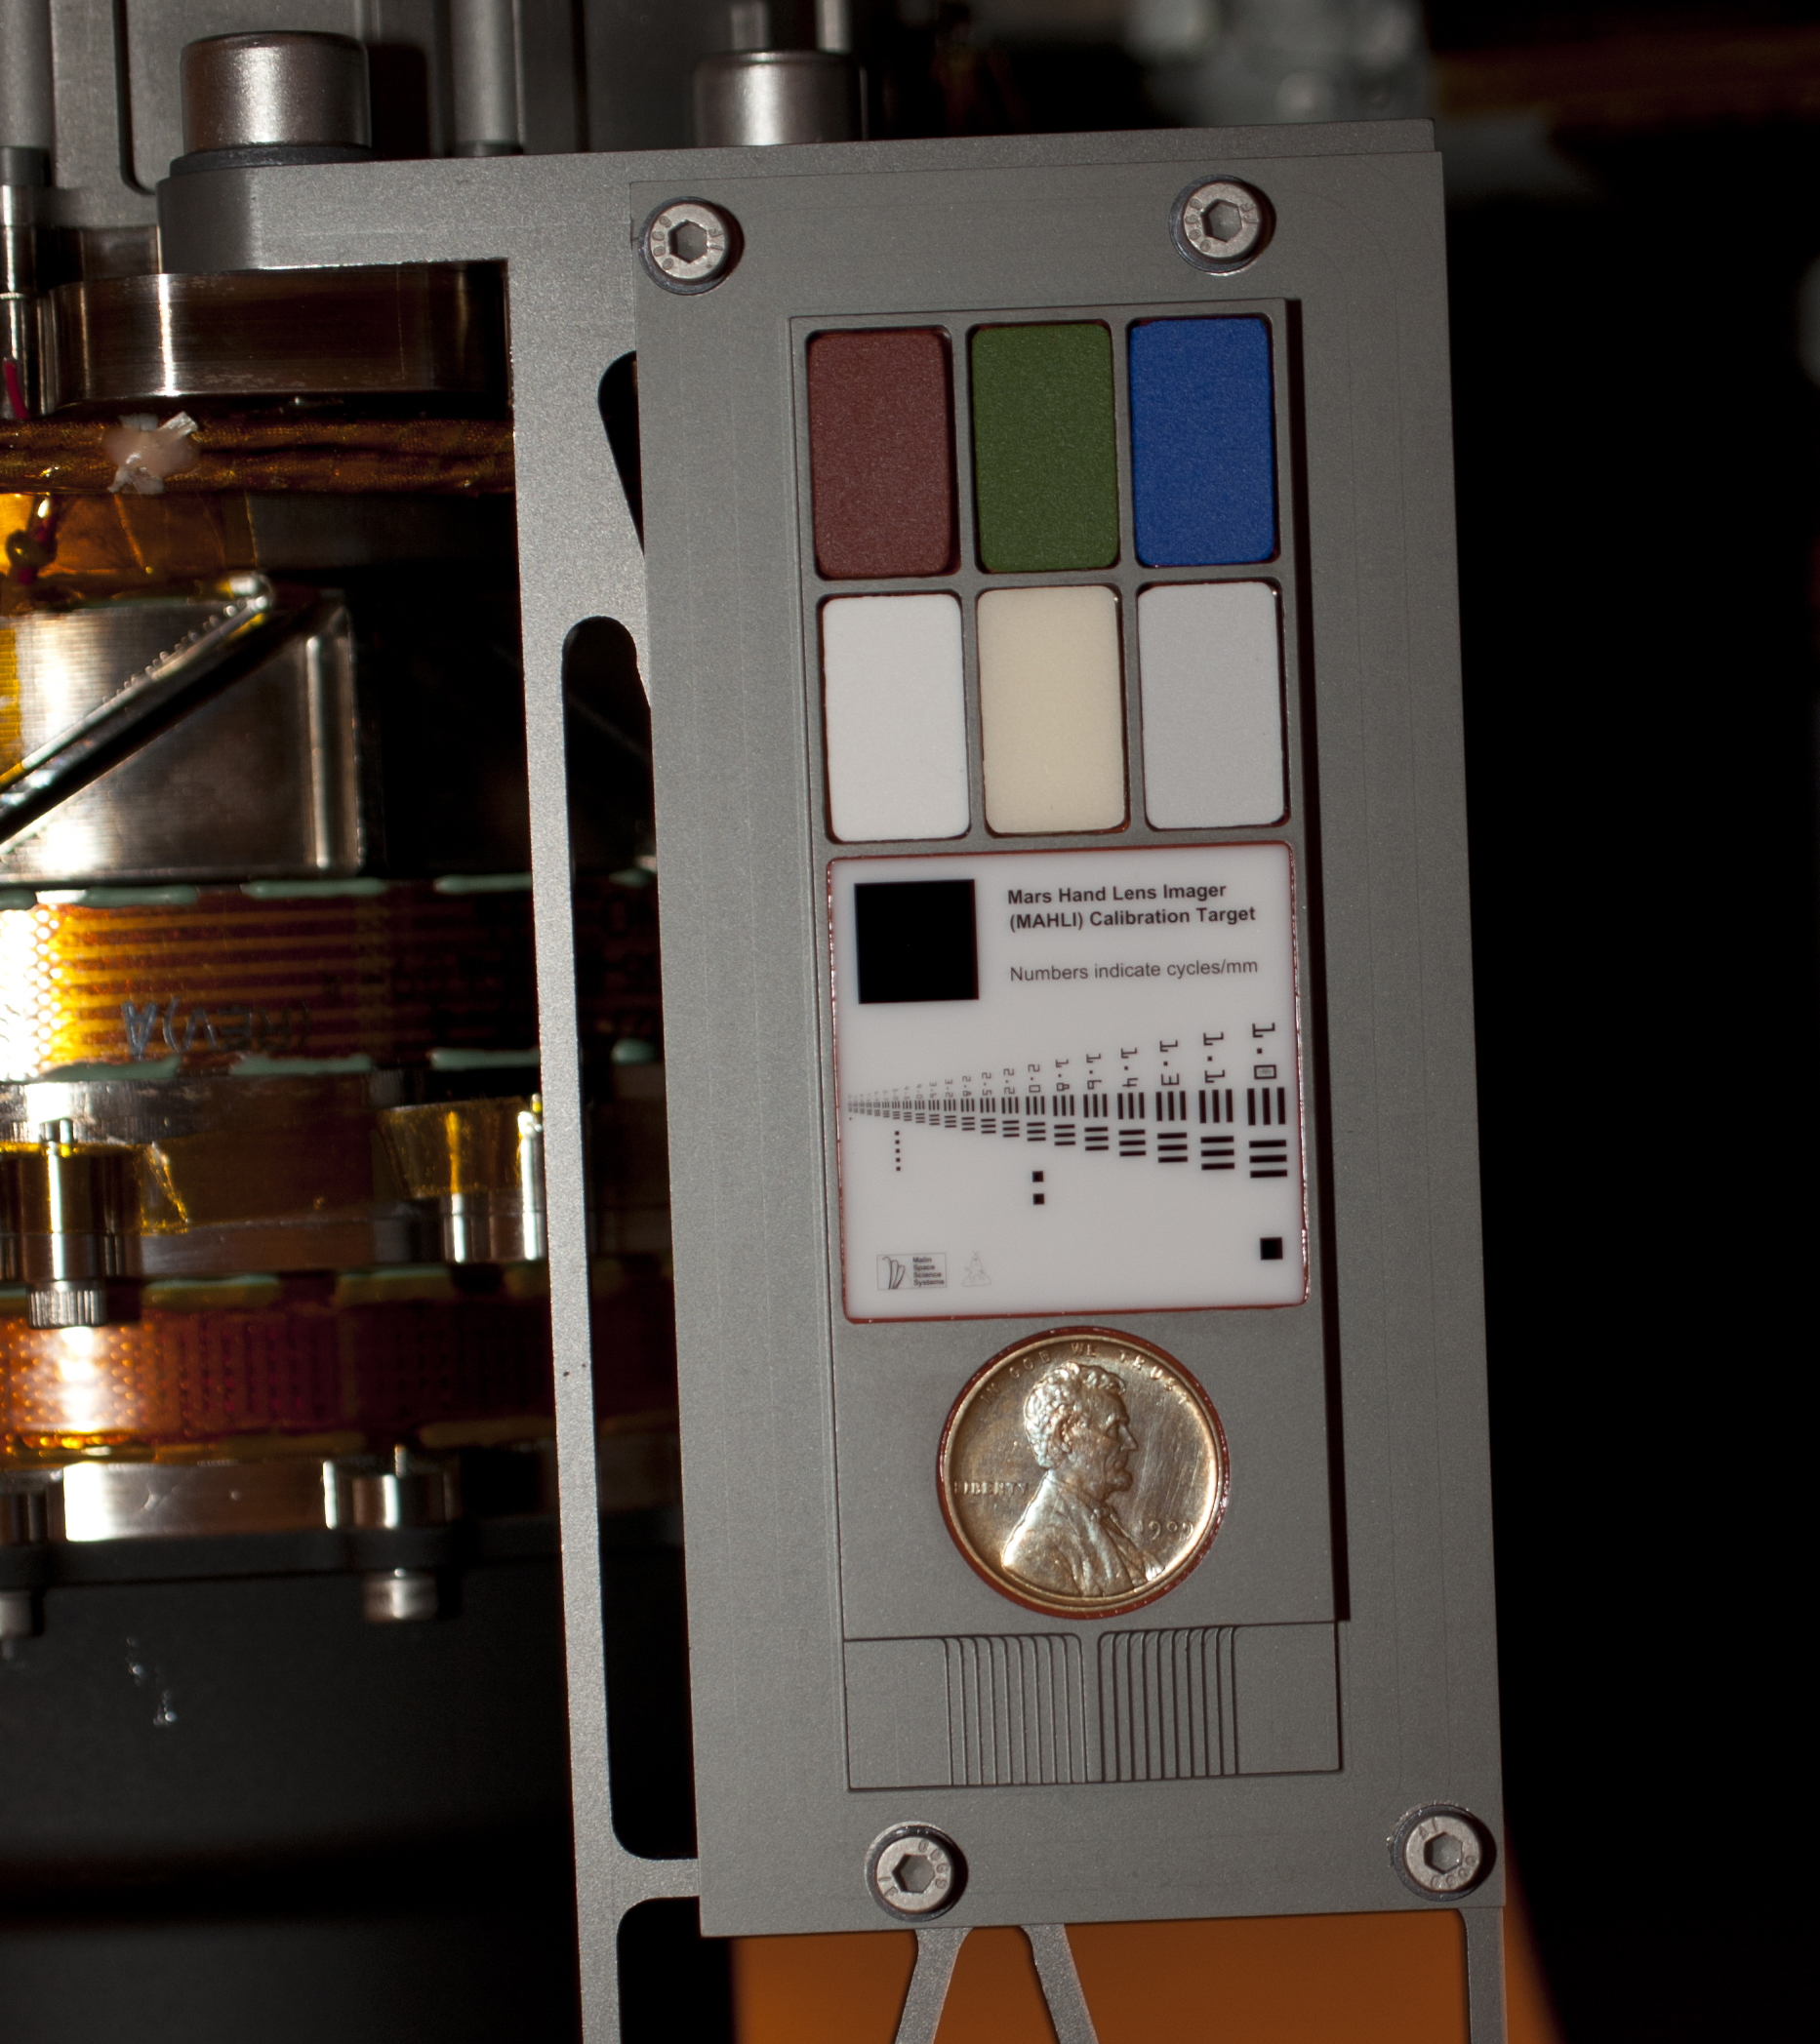
\includegraphics[width=7cm]{../images/curiosity_calibration_chart.jpg}
		\caption{The camera calibration items attached to the mars rover, Curiosity}
		\label{fig:curiosity_calibration_chart}
	\end{figure} 
	\subsection{Image Analysis in Sports Science}
	The benefits of image analysis in sports science are most prevalent in the area of biomechanics. In most sports, an individual’s performance depends on a combination of physical fitness and acquired skills. In certain sports, such as motorsports, equipment is undeniably important although unless “driver-athletes” can cope with the stresses and strains of race conditions they are unlikely to achieve success regardless of the technical superiority of their vehicle \citep{klarica2001performance}.
	\\\\
	In such sports, the performance of cars, motorcycles, and even mountain bikes are predictable and measurable. They have all been designed and manufactured to be as fast as possible within the rules laid down by the sport’s governing body so it is important to continually analyse and fine tune their setup by changing tires or adjusting suspension. Doing so seeks out the marginal gains that make the difference between gaining a place on the podium or not. As a result, performance cars and bikes are fitted with an array of sensors that constantly monitor critical aspects of performance such as engine temperatures or suspension \citep{segers2008analysis}. 
	\\\\
	Fitting sensors to humans without impairing their mobility is not quite so simple. To provide the best testing ground for fitness and technique, the participant should be unhindered and able to perform tasks without data capturing equipment getting in their way. Image analysis can get around such issues by utilising various techniques that can allow for stable and repeatable test situations while also providing a platform for reviewing the captured images. A study into bowling techniques in cricket used a mix of manual point picking and automated measuring from images to produce data such as the angle and speed of bowling deliveries as well as ball spin \citep{cricketimaging}. While the dataset was limited due to conflicts with the players’ training schedules, the results proved useful and were subsequently replicated in a pitching machine so that batsmen practised against more lifelike deliveries.
	\\\\
	A second study on the use of IA in showjumping \citep{jumpyhorses} made use of techniques similar to those used by Cook, Justham, and West. In this instance, the angles of the horse’s limbs were recorded and compared over a period of four months to analyse whether different training techniques delivered measurable improvements. Here, passive image analysis was chosen as the preferred technique as attaching sensors to the horse could have frightened the animal and almost certainly caused it to perform below par.
	\subsection{Using Image Analysis for Optimizing Mountain Bike Suspension}
Though image analysis has been used for calculations in many engineering and sports applications \citep{concreteanalysis, bridgecables}, it is relatively unused with mountain bike suspension with only Fox Racing Shox using the technology for setup purposes \citep{foxird}. The mobile application which Fox created is locked to \glspl{fork} and \glspl{shock} that the company manufacture though image analysis techniques are adaptable enough to be used on any suspension unit.
\\\\
By harnessing the image capturing and computing power of modern smartphones, image analysis can be applied to mountain bike suspension to produce a simple method of calculating a baseline setup for any suspension unit. The measurements and calculations required can be removed from the user's responsibility creating a simple and efficient method of generating a safe and reliable suspension setup.
	\newpage
	\section{Methodology}
	\subsection{Introduction}
	This chapter will give an outline of the methodologies used to complete the work identified in the previous chapters as well as the reasons for using these methods and alternatives which could have been used. The effectiveness of these methods can determine the success of the project so the chosen methods were required to reliable and manageable. A technical approach was identified for the most appropriate way to produce a solution to the problem identified and a project management approach was decided on so that the project could remain on track and meet the required deadline.
\subsection{Literature Review}
\subsection{Platform}
	As a proof of concept, the final product of this software project could take a variety of forms. Inline with current products on the market an application for Android could be produced which would demonstrate the capabilities of image analysis on a mobile device. Alternatively, the image analysis algorithm can be produced in the Python programming language as a script.
	\subsubsection{OpenCV}
		OpenCV is an open-source computer vision library created for a variety of platforms. Originally released by Intel in 1999 the library was intended as a research project to aid in CPU intensive visual applications. In 2012, the library was taken over by OpenCV.org, a non-profit organisation who maintain support and the documentation. Though the library is written in C and C++, modules are available for Python, Fortran, and the Android platform.
		\\\\
		This project will use OpenCV as it is widely accepted as the best, free computer vision library available and provides functions for the various processes this project will require. Additionally it is well supported and documented which will aid in the development process.
	\subsubsection{Experimentation}
		To further understand what may be required to produce both the Android and Python based approaches some basic experiments were carried out to compare the two and aid in deciding which method to use. For the Android experiments some example applications which are bundled with the OpenCV library were hand copied and run on a mobile device. This allowed their output and functionality to be seen as well as experience in using OpenCV on Android. For the Python based approach, tutorials from the site www.pyimagesearch.com created by Adrian Rosebrock were followed and run on a desktop computer.
		\\\\
		Appendix \ref{app:android_experiments} shows the experiments which were carried out on the android platform. It should be noted that, while all applications do not show compilation errors and were adjusted to work with the updated version of Android which the device was using, only two of the four experiments work successfully. Although a stack trace of the errors produced they are not descriptive about the cause of the error. This is due to how OpenCV works on the Android system.
		\\\\
		Alongside the Android Software Development Kit (SDK), Google provide a Native Development Kit (NDK) to allow modules which were not written in Java to be run on Android devices. The NDK understands various programming languages and applied a Java wrapper around them which is capable of extracting their functionality; this must be applied when using OpenCV on Android as it is written in C++. An artefact of using the NDK is that it cannot convert the stack trace produced by errors in the C++ module and after research into this issue it was found that it is difficult to rectify.
		\\\\
		The two working Android experiments do not operate as expected either. Shown in appendix \ref{app:android_experiments} the issues with each can be seen. Although steps were taken to rectify the orientation in the Hello CV experiment and the full-screen issue in both, any fix which was applied was not accepted by the system. Research and debugging of these faults did not produce any conclusions either.
		\\\\
		Appendix \ref{app:python_experiments} shows the experiments which were carried out using Python. These were much more successful than the Android experiments as they are all functional and work as expected.
		\\\\
		Included in appendix \ref{app:android_experiments} and \ref{app:python_experiments} as a comparison between the two methods are the number of files and lines of code required to create the program. There is a clear difference between the two methods. The Android method taking an average of 295 lines of code over 3 files to produce arguably less complex and less functional applications than is produced by Python's 21 lines of code over 1 file.
		\\\\
		Due to the difficulties when using OpenCV on Android and as the operating system is already a proven platform for mobile applications the decision has been made to produce a poof of concept for the image analysis in Python. This will allow the project to maintain focus on the analysis and algorithmic side of the problem as opposed to the portability. The decision also allows for more time to be spent making the program functionally stable which will serve as a better demonstration of the solution.
\subsection{Project Management}
	\subsubsection{Agile Development}
		Introduced in 2001 with the writing of the Agile manifesto \citep{beck2001manifesto}, agile development methodologies focus on high quality software products over the rigorous design based structure of traditional methods. By utilising various techniques such as stand-up meetings, a strong customer focus, and sprint cycles, agile has become widely adopted in industry and has been proven to produce successful projects \citep{state_of_agile_2015}.
		\\\\
		There are multiple agile methodologies (XP, Scrum, DSDM) all with their own principles and techniques however it is commonplace for a company to create their own development method which picks items from each to tailor to their needs. As this is a solo project with no customer then one set methodology will not be used, instead a variety of methods which will aid the management of the project and increase the efficiency of the development process have been selected. These will be outlined in the following sections.
		\paragraph{Requirements Analysis}
		\paragraph{MoSCoW}
			First used in the DSDM agile framework, MoSCoW analysis or prioritisation is the process of taking the requirements of a software product and placing them into one of four categories; must, should, could, and won't have. These deliverables may be prioritised for the entire project or for individual sprint cycles depending on the size and manageability of the project.
			\\\\
			MoSCoW was created to provide customers a better understanding of software requirements. Opposed to using high, medium, and low priorities MoSCoW is more descriptive of what the prioritisation means for the software project. From a development point of view the prioritisation process allows developers to focus on the core requirements of the project first, creating a viable software solution early on with extra features being added later if the resources are available.
			\\\\
			This project will use MoSCoW to prioritise the requirements identified using the requirements analysis technique allowing the development process to complete the requirements in the correct order. This will ensure that the core aspects of the solution are implemented first creating a successful project early and allowing it to improve as time allows.
		\paragraph{Sprint Cycles}
			Used by Scrum development teams, a sprint is a timeboxed effort of work scheduled to take between one week and one month. At the start of a sprint goals are chosen from the project requirements which are to be completed by the end of the sprint. When a sprint is complete a retrospective is carried out by the development team to discuss what went well, what didn't, and how this can be rectified for the next sprint.
			\\\\
			This project will use sprints in the same manner as an agile development team as this will allow easier completion of requirements and management of the development process. Using sprints will ensure the time allotted for development is used effectively which will lead to a higher quality product at the end of the project.
			\\\\
			As mentioned previously, MoSCoW prioritised requirements will be selected at the start of each sprint cycle to set objectives the work which will be carried out. Each cycle will aim to complete all of the must have requirements and the majority of should and could haves. At the end of each cycle a retrospective will be carried out which will re-prioritise the uncompleted requirements based on how successful the sprint cycle was. This means requirements may be promoted or demoted respectively.
	\subsubsection{Version Control}
		Large software projects produce multiple files of code and documentation which are vital and must be kept safe. Were the files to be lost then the project would be delayed or drawn to a close as the time and resources may not be available to recreate the lost data. To combat this any data relating to the project must be backed up, preferably on a cloud based system, to avoid loss and allow the project to continue should anything happen to the local copy of the data.
		\\\\
		For this project the Git \gls{vcs} will be used. Git provides free use of a cloud based repository to store any files relating to a project and allows for work to be carried out locally by cloning the repository on a computer. However \glspl{vcs} also enable the management of the previous versions of files including information such as the individual changes made, when those changes were made, and who made the changes. This is a powerful tool as it means the various sections of the project can be experimented on without the risk of damaging the project; if a change is unsuccessful then the repository can be reverted to a functional point.
		\\\\
		The web service used to host the repository will be github.com. This site was chosen as it provides unlimited free repositories as well as simple repository management tools. The website also provides issue tracking functionality; though they are not issues, each feature will be added as an entry in the issue tracker. The reason for this is that all features will have a unique identification and description which commits to the repository can be placed against. This is useful for project management reasons as then each feature's stage and completeness can be monitored to ensure the project's success.
		\\\\
		Alternative \glspl{vcs} are available, for example Microsoft's Team Foundation Server or Perforce, however these are limited under free licences or locked to certain development environments. The accessibility and ease of use provided by Git makes it the optimum \gls{vcs} to use for this project. 

	\newpage	
	\section{Results}
	\newpage
	\section{Critical Evaluation}
	\newpage
	\section{Conclusion}
	\newpage
	\bibliography{bibliography}	
	\newpage
	\printacronyms
	\printglossary[type=main]
	\clearpage
	\appendix
	\thispagestyle{empty}
	\newgeometry{margin=1cm}
	\begin{landscape}
		\section{Android Experiments}\label{app:android_experiments}
		\subsection{Table of Android Experiments}
		\begin{table}[h!]
			\centering
			\label{tab:android_experiments}
			\begin{tabular}{|l|p{0.4\textwidth}|l|p{0.4\textwidth}|r|r|}
				\hline
				\bfseries Experiment&\bfseries Purpose&\bfseries Functiona?l&\bfseries Issues&\bfseries Files&\bfseries LOC\\
				\hline
				Hello CV&
				\begin{itemize}[noitemsep,topsep=0pt,parsep=0pt]
					\item{Introduction to the android OpenCV library}
					\item{Displays camera feed with fps}
				\end{itemize}&
				Yes&
				\begin{itemize}[noitemsep,topsep=0pt,parsep=0pt]
					\item{Not fullscreen}
					\item{Incorrect orientation}
				\end{itemize}&
				2&
				101\\
				\hline
				15Tile&
				\begin{itemize}[noitemsep,topsep=0pt,parsep=0pt]
					\item{Sliding tile game}
					\item{Uses camera feed as puzzle}
				\end{itemize}&
				Yes&
				\begin{itemize}[noitemsep,topsep=0pt,parsep=0pt]
					\item{Not fullscreen}
				\end{itemize}&
				3&
				492\\
				\hline
				Blob Detection&
				\begin{itemize}[noitemsep,topsep=0pt,parsep=0pt]
					\item{Demonstrates blob detection}
					\item{Runs blob detection on tapped area from camera}
				\end{itemize}&
				No&
				\begin{itemize}[noitemsep,topsep=0pt,parsep=0pt]
					\item{Crash on screen tap}
				\end{itemize}&
				3&
				311\\
				\hline
				Face Detection&
				\begin{itemize}[noitemsep,topsep=0pt,parsep=0pt]
					\item{Detects faces in camera view}
					\item{Puts boundary around detected faces}
				\end{itemize}&
				No&
				\begin{itemize}[noitemsep,topsep=0pt,parsep=0pt]
					\item{Crash on load}
				\end{itemize}&
				3&
				279\\
				\hline
			\end{tabular}
		\end{table}
	\end{landscape}
	\restoregeometry
	\subsection{Hello CV}
	\inputminted{java}{../code/android/hello_cv/MainActivity.java}
	\subsection{15tile}
	\inputminted{java}{../code/android/15tile/MainActivity.java}
	\inputminted{java}{../code/android/15tile/PuzzleProcessor.java}
	\subsection{BLOB Analysis}
	\inputminted{java}{../code/android/blob_analysis/ColorBlobDetectionActivity.java}
	\inputminted{java}{../code/android/blob_analysis/ColorBlobDetector.java}
	\subsection{Face Detection}
	\inputminted[]{java}{../code/android/face_recognition/DetectionBasedTracker.java}
	\inputminted[]{java}{../code/android/face_recognition/FrActivity.java}
	\clearpage
		\thispagestyle{empty}
		\newgeometry{margin=1cm}
		\begin{landscape}
			\section{Python Experiments}\label{app:python_experiments}
			\subsection{Table of Python Experiments}
			\begin{table}[h!]
				\centering
				\label{tab:python_experiments}
				\begin{tabular}{|l|p{0.4\textwidth}|l|p{0.4\textwidth}|r|r|}
					\hline
					\bfseries Experiment&\bfseries Purpose&\bfseries Functiona?l&\bfseries Issues&\bfseries Files&\bfseries LOC\\
					\hline
					Find Game&
					\begin{itemize}[noitemsep,topsep=0pt,parsep=0pt]
						\item{Identify red game cartridge out of 3}
						\item{Displays boundary around correct part of image}
					\end{itemize}&
					Yes&
					N/A&
					1&
					18\\
					\hline
					Threshold Methods&
					\begin{itemize}[noitemsep,topsep=0pt,parsep=0pt]
						\item{Demonstrates various thresholding methods on an image}
						\item{Original image text unreadable but clear after techniques are applied}
					\end{itemize}&
					Yes&
					N/A&
					1&
					14\\
					\hline
					Image Operations&
					\begin{itemize}[noitemsep,topsep=0pt,parsep=0pt]
						\item{Moves parts of an image to other locations using arrays}
						\item{Demonstrates how pixel data is stored}
					\end{itemize}&
					Yes&
					N/A&
					1&
					15\\
					\hline
					Distance to Camera&
					\begin{itemize}[noitemsep,topsep=0pt,parsep=0pt]
						\item{Calculates distance to the camera from an identified object}
						\item{Displays various distances using 3 images}
					\end{itemize}&
					Yes&
					N/A&
					1&
					38\\
					\hline
				\end{tabular}
			\end{table}
		\end{landscape}
		\restoregeometry
		\subsection{find\_game.py}
		\inputminted{python}{../code/python/find_game.py}
		\subsection{thresholding.py}
		\inputminted{python}{../code/python/thresholding.py}
		\subsection{img\_ops.py}
		\inputminted{python}{../code/python/img_ops.py}
		\subsection{distance\_to\_camera.py}
		\inputminted{python}{../code/python/distance_to_camera.py}
\end{document}